\documentclass[12pt,a4paper]{report}

%Image-related packages
\usepackage{graphicx}
\usepackage{subcaption}
\usepackage[export]{adjustbox}

%Style
\setlength{\parskip}{1em plus 0.25em minus 0.25em}
\renewcommand{\baselinestretch}{1.5}

%Table of contents, figures, tables
\usepackage[nottoc]{tocbibind}

\usepackage{hyperref}
\usepackage{xcolor}
\hypersetup{
    colorlinks,
    linkcolor={blue!50!black},
    citecolor={blue!50!black},
    urlcolor={blue!80!black}
}

\usepackage{cite}
\usepackage{chemformula}
\usepackage{appendix}

%Table style
\usepackage{multirow}
\usepackage{tabularx}
\setlength{\arrayrulewidth}{0.2mm} %The thickness of the borders
\setlength{\tabcolsep}{18pt} %The space between the text and the left/right border
\renewcommand{\arraystretch}{1.5} %The height of each row
\usepackage{colortbl} %Table cell colour

%Header & footer
\usepackage{fancyhdr}

%Redefines the /today command
\renewcommand{\today}{\ifcase \month \or January\or February\or March\or April\or May%
\or June\or July\or August\or September\or October\or November\or December\fi\:%
\number \year}

%Glossary
\usepackage{glossaries}
\makeglossaries

\newglossaryentry{ghg}
{
    name=GHG,
    description={Greenhouse gas}
}

\newglossaryentry{co2}
{
    name=\ch{CO2},
    description={Carbon dioxide}
}

\newglossaryentry{eu}
{
    name=EU,
    description={European Union}
}

\newglossaryentry{pv}
{
    name=PV,
    description={Photovoltaic}
}

\newglossaryentry{ee}
{
    name=EE,
    description={Energy efficiency}
}

\newglossaryentry{sd}
{
    name=SD,
    description={Sustainabe Development}
}

\newglossaryentry{re}
{
    name=RE,
    description={Renewable energy}
}

\newglossaryentry{sems}
{
    name=SEMS,
    description={Smart energy management system}
}

\newglossaryentry{nape}
{
    name=NAPE,
    description={The National Action Plan on Energy Efficiency}
}

\newglossaryentry{dr}
{
    name=DR,
    description={Demand response}
}

\newglossaryentry{hp}
{
    name=HP,
    description={Heat pump}
}

\newglossaryentry{rs}
{
    name=RS,
    description={Recommender systems}
}

\newglossaryentry{nl}
{
    name=NL,
    description={Natural language}
}

\newglossaryentry{iv}
{
    name=IV,
    description={Information Visualisation}
}

\begin{document}

\begin{titlepage}

\begin{center}

\vspace*{-1cm}

\begin{figure}[h]
  \begin{subfigure}{0.50\textwidth}
    
\includegraphics[width=0.8\linewidth, left]{Images/siegen.png}
  \end{subfigure}
  \begin{subfigure}{0.49\textwidth}
    
\includegraphics[width=0.8\linewidth, right]{Images/isi.jpeg}
  \end{subfigure}
\end{figure}

\vfill

%\textbf{\large Research Proposal}\\[10pt]
{\Large \bf Filling the Information Gap of House Owners and Technologies: A Design Case Study of a smart recommender for home energy system} \\

\vfill
In partial fulfilment of the requirement for the degree of\\
{\large \bf MASTER OF SCIENCE}\\
in\\ 
{\large \bf Human Computer Interaction } \\
{\em by} \\
{\large \bf Yanwei Miao} \\
{\large \bf (1627738)}\\

Under the supervision of \\
{\bf \large Prof. Dr. Gunnar Stevens} \\
{\bf \large Dr. Songmin Yu} \\

\vfill

{\it \large \today}

\end{center}

\end{titlepage}

\clearpage
\pagenumbering{roman} \setcounter{page}{2}
\begin{center}
{\Large{\bf{ABSTRACT}}}
\end{center}

\noindent

Climate change is a threat to the environment and society. 
Evidences show human behaviours are the main contributions to the global warming. 
There is an ergent need to slow down the process of global warming. 
The goal has been raised in the Paris Agreement.
And at the EU level, there are 2 goals that should be achieved by 2030 and 2050.  

\clearpage
\tableofcontents
\clearpage
\listoffigures
\listoftables

\newpage
\clearpage % Start a new page

\noindent

{\Huge{\bf{Notations and Abbreviations}}}\
\\[6pt] 

\newglossaryentry{ghg}
{
    name=GHG,
    description={greenhouse gas}
}

\newglossaryentry{co2}
{
    name=\ch{CO2},
    description={carbon dioxide}
}

\newglossaryentry{eu}
{
    name=EU,
    description={European Union}
}

\printglossaries

\newpage

\pagenumbering{arabic}
\setcounter{page}{1}

\chapter{Background} 

Human-induced climate change is causing dangerous and widespread disruption in nature and affecting the lives of billions of people around the world \cite{ipcc}. 
To tackle climate change and its negative impacts, the historic Paris Agreement sets long-term goals to guide all nations to substantially reduce global greenhouse gas (\gls{ghg}) emissions to limit the global temperature increase to 2 degrees Celsius in this century \cite{paris}. 
On European Union (\gls{eu}) level, 
“Energy 2020. A strategy for competitive, sustainable and secure energy”, published in November 2010, and “Energy Roadmap 2050”, published at the end of 2011, are the most important strategy papers currently, pointing the direction for energy developments in the \gls{eu} \cite{roadmap}. 
The aim is to confirm Europe's commitment to lead in global climate action and to present a vision that can lead to achieving net-zero \gls{ghg} emissions by 2050 through a socially-fair transition in a cost-efficient manner \cite{clean}. 

%To achieve these goals, two central strategies are pursued by the \gls{eu} and its Member States concerning the energy system \cite{2050}: 

%\begin{enumerate}
%  \item Enhancing energy efficiency (EE). 
%  \item Decarbonizing energy supply, 
%  in particular via large diffusion 
%  and wide-use of renewable energy sources.
%\end{enumerate}

\section{Energy transition}

\subsection{Energy demand}

\subsection{Energy supply}

\subsection{Infrastructure}

%In 2019, 80.9\% of our total energy supply still depended on burning fossil fuels, namely 26.8\% coal, 30.9\% oil and 23.2\% natural gas \cite{iea}. 
%Nonetheless, investments into low-carbon power generation accounted for 15\% recently are expected to rise to more than 30\% by 2030, corresponding to a quadrupling in absolute volumes \cite{shift}. Solar, wind, and the investments for enabling the integration of these technologies to the grid dominate the investments into low-carbon power generation \cite{shift}. 

%\subsection{Societal trends}

%Previous research has shown that in many areas energy efficiency gains were counteracted by societal trends that increased corresponding activities, leading to much smaller decreases (or even increases) of energy demand than technologically feasible \cite{2050}. 
%Therefore, it is important to access current and (foreseeable) future societal trends concerning the impact that they might have on future energy demand \cite{2050}.

%Climate change can only be tackled if people actively engage, as consumers and as citizens \cite{clean}. 

\section{The newTRENDs Project}

The aim of NewTRENDs is to increase the qualitative and quantitative understanding of impacts of New Societal Trends on energy consumption and to improve the modelling of energy demand, energy efficiency and policy instruments \cite{fraunhofer}. 

\subsection{Concept}

%The newTRENDs project develops the analytical basis for a ``2050 Energy Efficiency Vision" by considering New Societal Trends in energy demand modeling \cite{newtrends}.

With increasing renewable generation integrated into the power system, supply-side fluctuations must be balanced by demand-side flexibility. 
Electrification and demand response (DR) are becoming increasingly relevant to the heating transition of buildings, which demands the diffusion of

\begin{itemize}
  \item heat pumps (HPs),
  \item photovoltaic (PV) and energy storage (e.g., battery and hot water tank),
  \item smart energy management systems (SEMSs).
\end{itemize}

Combining the three technologies is also beneficial from an individual household (or building) perspective. The household can optimize the heat pump operation to reduce energy costs by saving energy in the tanks or pre-heat the building when the electricity price is lower. Besides, the energy-saving benefit could be further increased with PV and battery system.
From a market perspective, DR flexibility and PV generation also facilitate the concept of "energy community". The households can trade electricity with each other (peer-to-peer, P2P) within a local micro-grid or even trade with the other side of the country through the national grid, depending on the infrastructure, business model, and policies. In addition, households can also buy the services from an "aggregator", who bundles and manages the flexibility of small consumers and producers and participate in the market activities (Kerscher and Arboleya 2022). 
Promoted by the declining costs of technologies and support policies, more and more household "consumers" are expected to become "prosumers" (with PV) and "prosumagers" (plus energy storage and SEMS) (Fereidoon Sioshansi 2019).

\subsubsection{FLEX models}

The FLEX-Operation and FLEX-Community models were built to improve the building modeling suite and to analyze the societal trends of prosumaging and energy communities.
The figure \ref{fig:flex} shows how FLEX interacts with other bottom-up models involved in the newTRENDs project.

\begin{figure}[h]
  \centering
  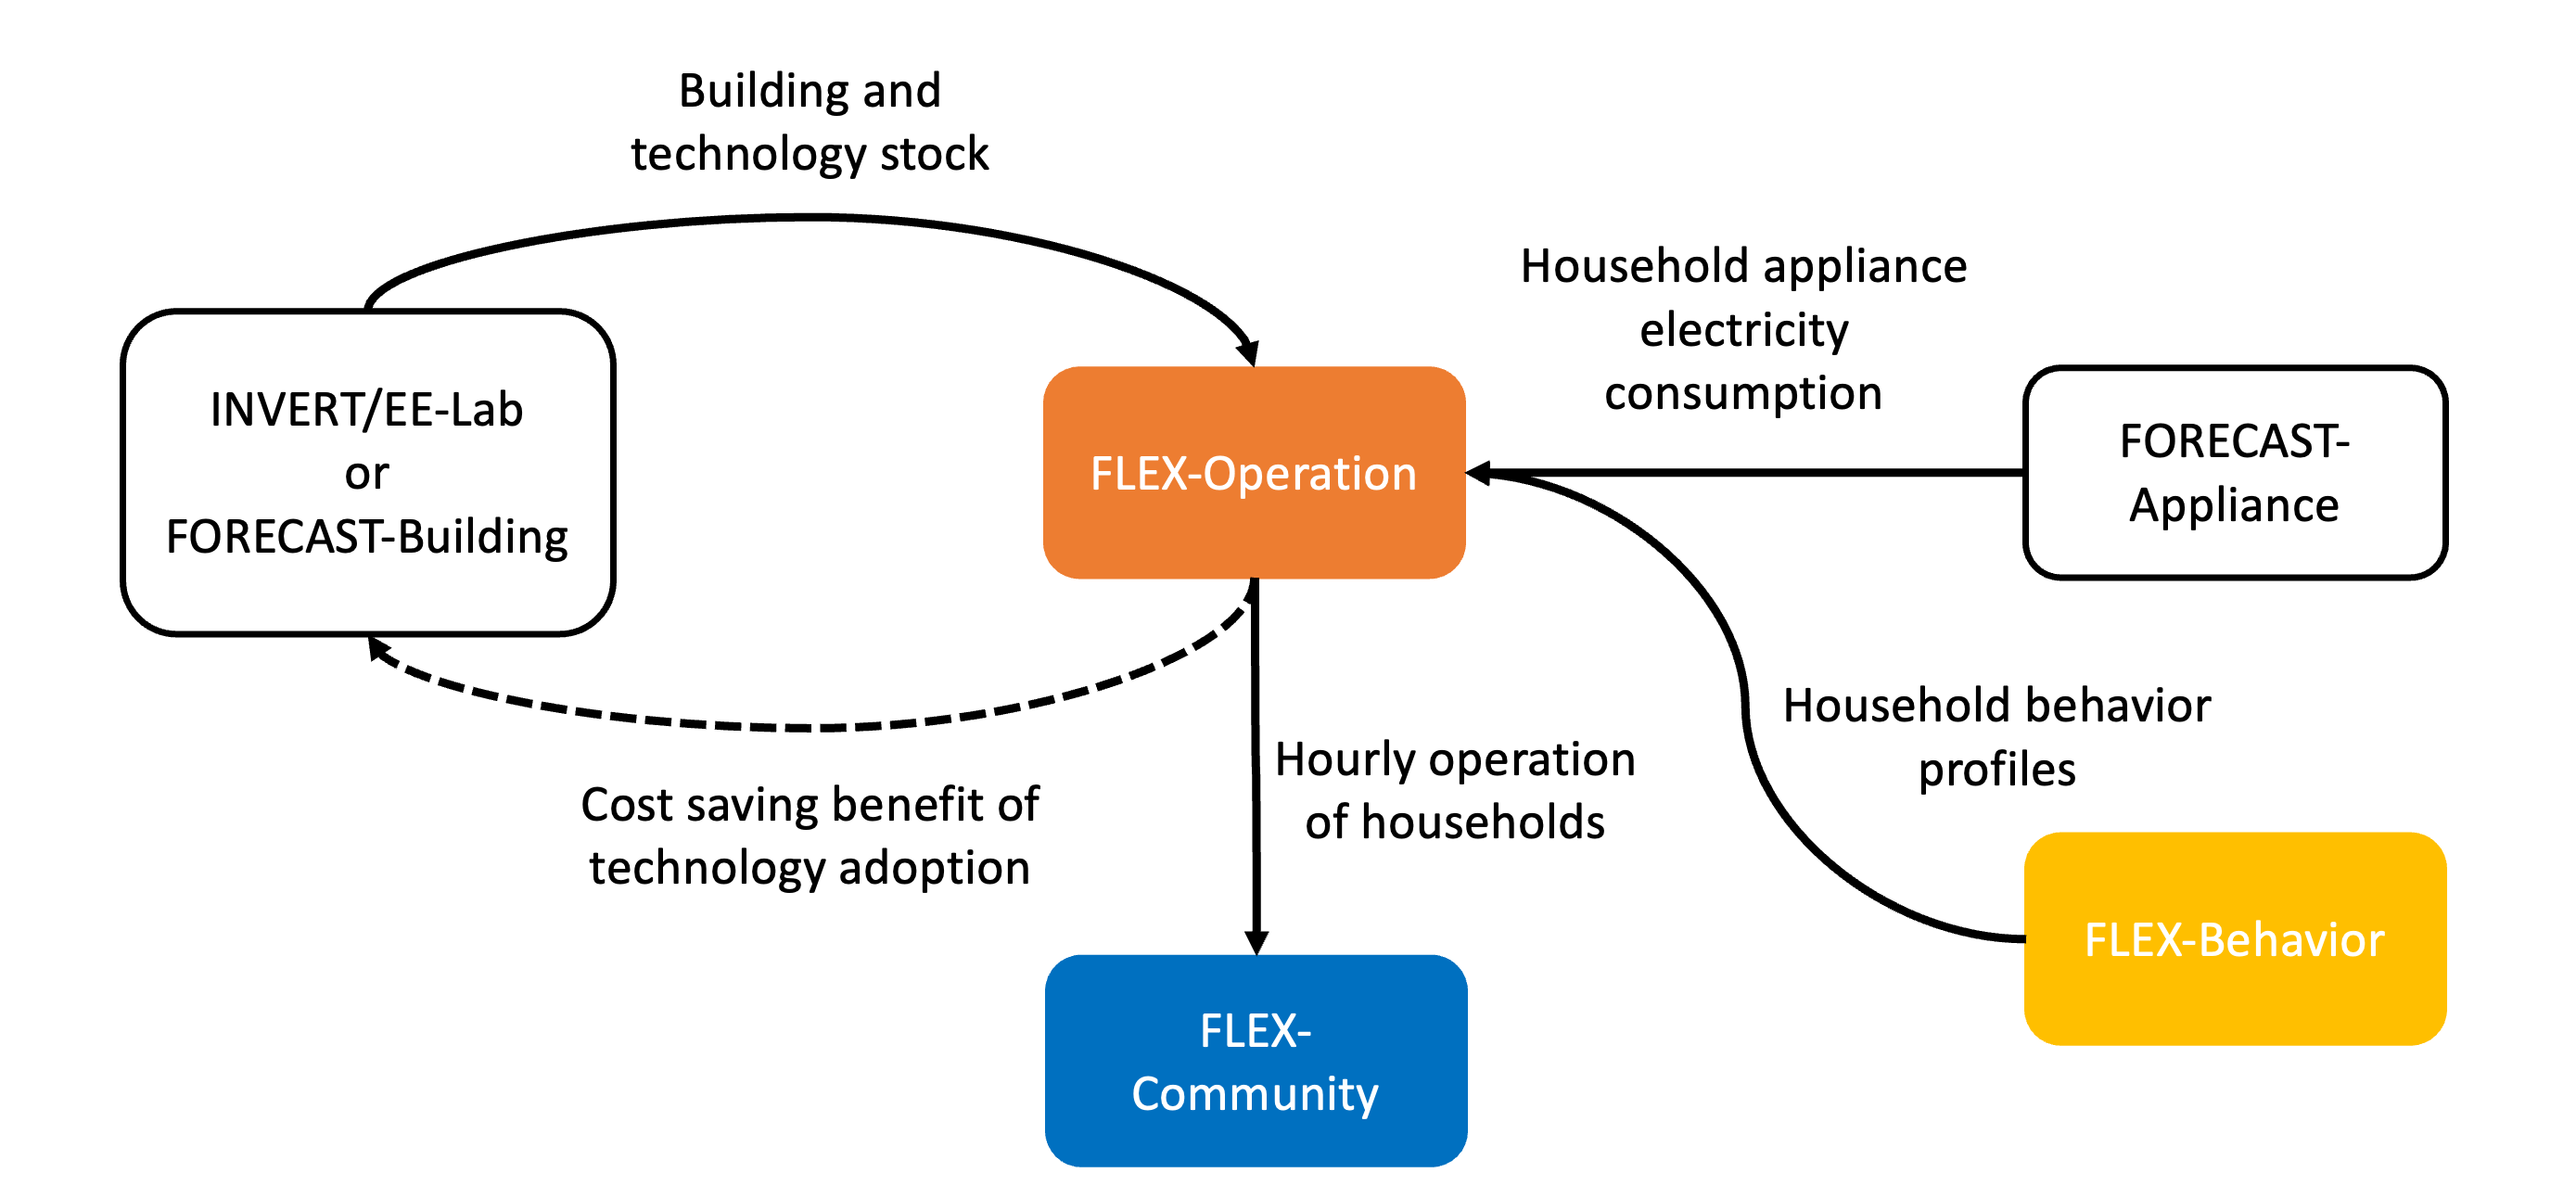
\includegraphics[width=\textwidth]{Images/flex.png}
  \caption{FLEX modeling suite}
  \label{fig:flex}
\end{figure}

INVERT/EE-Lab and FORECAST-Appliance are the two models that can cover the energy consumption of residential buildings. The two models complement each other and cover the total energy consumption of households. 
However, both INVERT/EE-Lab and FORECAST-Appliance calculate the energy consumption at the annual resolution and cannot model the prosumaging behavior and energy community, which requires an hourly resolution to consider the impact of household behavior, PV generation, and energy storage (thermal and battery) on energy consumption. In this regard, we developed the FLEX- Operation and FLEX-Community models to improve the building modeling suite and support relevant policy analysis.

\subsubsection{FLEX-Community}

FLEX-Community models the operation of an energy community, i.e., household interaction, aggregator optimisation. 
It can be applied to support the aggregators designing and evaluating business models, as well as making investment decisions, for example, the self-owned battery, PV panels, etc.

\subsubsection{FLEX-Behavior}

FLEX-Behavior models the behavior (activity profile) of households' and corresponding load profiles. 
It generates the hourly activity and energy demand profile of a pre-defined individual household. 
The results include

\begin{enumerate}
  \item appliance electricity demand,
  \item domestic hot water demand,
  \item driving profile, and
  \item building occupation.
\end{enumerate}

\subsubsection{FLEX-Operation}

FLEX-Operation models the energy system operation of an individual household in hourly resolution.  
It calculates the energy consumption of each representative building, including operation of technologies (e.g., battery, PV, heat pump, etc.) and load profiles in hourly resolution.

Data is considered by the model

\begin{itemize}
  \item building,
  \item heating system (heat pump, fuel-based boiler, electric heater),
  \item thermal storages for space heating and domestic hot water,
  \item space cooling technology,
  \item PV,
  \item battery, and
  \item electric vehicle.
\end{itemize}

\begin{figure}[h]
  \centering
  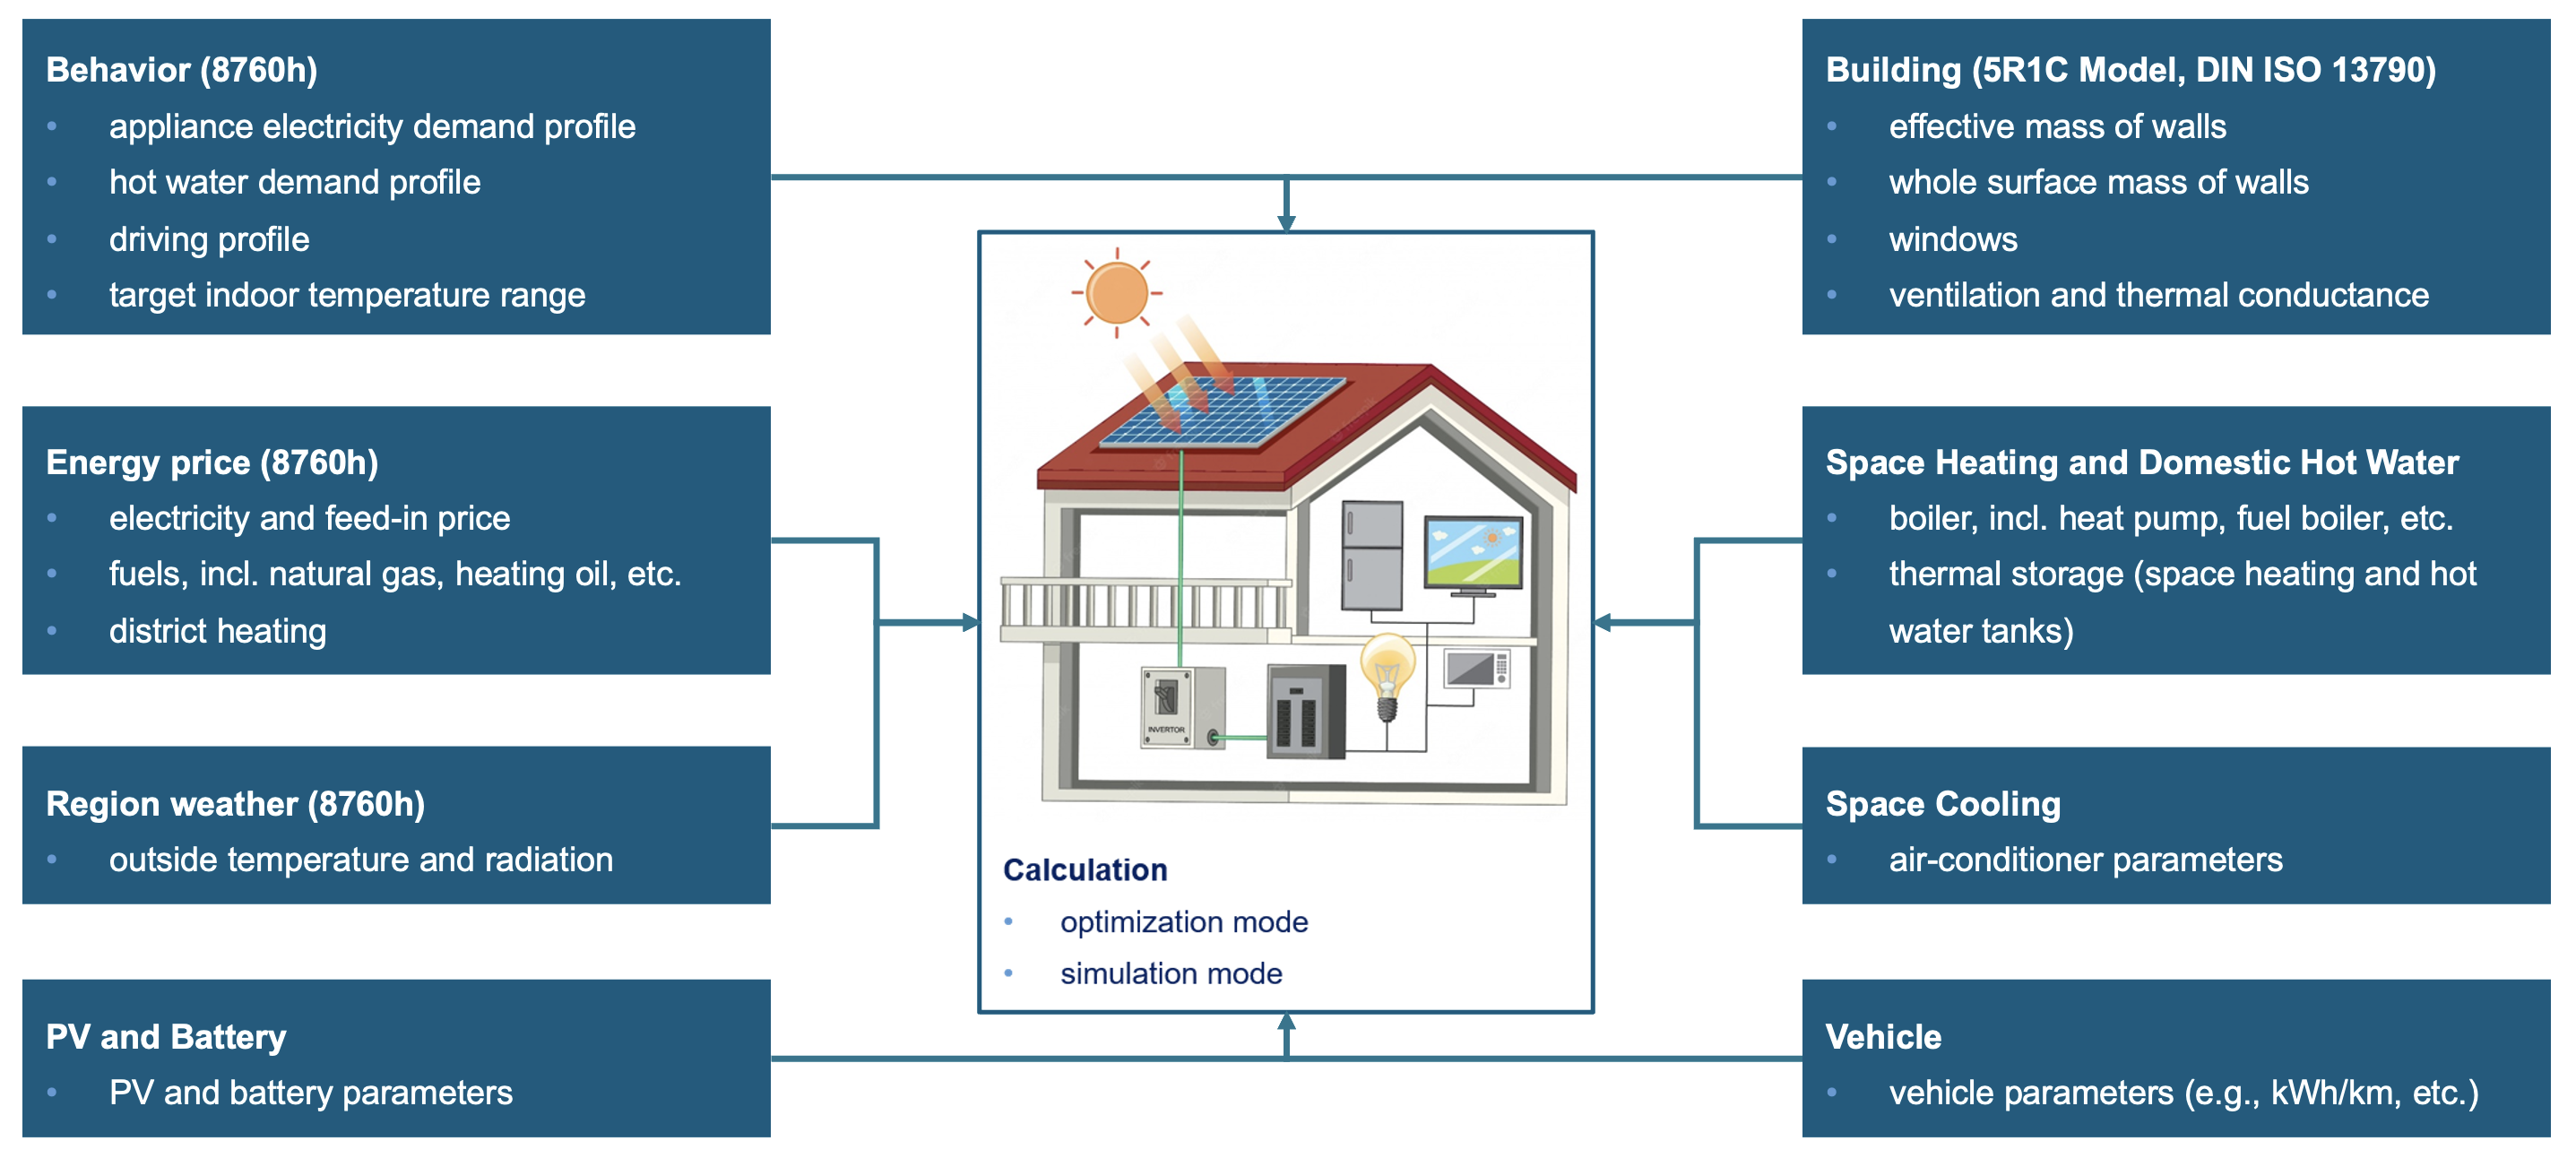
\includegraphics[width=\textwidth]{Images/flex-operation.png}
  \caption{FLEX-Operation}
  \label{fig:flex-operation}
\end{figure}

\section{Motivations}

As a part of the newTRENDs project, 
the proposed thesis will focus solely on the implementation of the FLEX-Operation model.  
By employing the model to 
suggest reliable, cost-effective energy optimisation solutions 
while giving households with comparable predicted statistics on their energy consumption for the time frame. 
Despite the fact that the model primarily responds to societal trends for 2030, 
which means it provides more flexible suggestions when a household already owns a photovoltaic (\gls{pv}) system, 
this could be as well an opportunity to nudge the European households who currently rely on other energy resources
to switch to renewable energy when feasible. 
And it will be beneficial not only to the environment but also to consumers. 

\subsection{Research gaps and questions}

There is a lack of case study research of promoting energy optimisation solutions. 
The aim of this proposed thesis is to design and develop a user-friendly web application for recomanding energy optimisation solutions.

The following criteria should be taken into account while building a software application from a user's perspective: 

\begin{itemize}
  \item It should be easy and effortless for using. 
  \item The interactions should be intuiative. 
  \item The recommandations should be clear explained to users. 
\end{itemize}

Objectives: 

\begin{itemize}
  \item Investigate the data of the FLEX-Operation model to build an energy optimisation recommendation system.
  \item Determine the typical European household types. 
  \item Design the web application with user-centred approaches. 
  \item Use data visualisation techniques to provide explainable suggestions. 
  \item Develop the frontend and backend web application. 
  \item Evaluate the explainability of the smart energy optimisation recommender at the user level and measuring the impact of the households perceptions towards energy optimisation solutions. 
  \item Allow long-term event tracking for iteration. 
\end{itemize}

Resaerch questions:

\begin{enumerate}
  \item What are the data required by the FLEX-Operation model from households? 
  \item What are the typical European household profiles? 
  \item How to build a trustworthy and user-friendly energy optimisation recommendation system? 
\end{enumerate}

\colorbox{orange}{Is there any literature review to add?}
\chapter{Methodology} 

The methodology adopted in this study is based on the Design Case Studies framework. 
The pre-study phase will begin by conducting a comprehensive review of the literature to identify best practices for providing households with personalised and professional home energy system recommendations, as well as techno-economic assessments.
Based on the findings from the pre-study, I will then design the interfaces of the intervention. 
The interfaces will be developed to provide an intuitive and user-friendly experience that can easily be understood by households. 
Following the development phase, real users will be invited to use the intervention, and feedback will be collected both qualitatively and quantitatively. 
The qualitative data will be collected through interviews with participants, while the quantitative data will be collected through surveys. 
Finally, the collected data will be analysed to evaluate households thoughts about the recommendations and energy technologies. 
The entire process will be documented and reported in the form of a thesis. 

\chapter{Supervision agreements and time planning} 

Introductory lines...

\section{Justification for 30 ECTS}

Research + design + develop

\section{Supervision}

This master thesis project will be supervised by 
Prof. Dr. Gunnar Stevens (\href{mailto:gunnar.stevens@uni-siegen.de}{gunnar.stevens@uni-siegen.de}) and 
Dr. Songming Yu (\href{mailto:songmin.yu@isi.fraunhofer.de}{songmin.yu@isi.fraunhofer.de}).  

\section{Time planning}

Some text\dots \\

\begin{table}[h]
    \begin{center}
        \begin{tabular}{ | p{0.05\linewidth} | p{0.8\linewidth} | }
        \hline 
        1 & \cellcolor{green!10!orange}Investigate the data of the FLEX-Operation model to build an energy optimisation recommendation system. \\
        \hline 
        2 & \cellcolor{green!20!orange}Determine the typical European household types. \\
        \hline 
        3 & \cellcolor{green!30!orange}Design the web application with user-centred approaches. \\
        \hline 
        4 & \cellcolor{green!40!orange}Use data visualisation techniques to provide explainable suggestions. \\
        \hline 
        5 & \cellcolor{green!50!orange}Develop the frontend and backend web application. \\
        \hline 
        6 & \cellcolor{green!60!orange}Evaluate the explainability of the smart energy optimisation recommender at the user level and measuring the impact of the households perceptions towards energy optimisation solutions. \\
        \hline
        7 & \cellcolor{green!70!orange}Allow long-term event tracking for iteration. \\
        \hline 
        \end{tabular}
        \caption{Objectives}
        \label{tab:objectives}
    \end{center}
\end{table}

\renewcommand{\arraystretch}{1.2}
\begin{table}[h]
    \begin{center}
        \begin{tabular}{ c c c c c c c c }
        & 1 & 2 & 3 & 4 & 5 & 6 & 7 \\ 
        w1  & \cellcolor{green!10!orange} \\  
        w2  & \cellcolor{green!10!orange} \\ 
        w3  &   & \cellcolor{green!20!orange} \\ 
        w4  &   & \cellcolor{green!20!orange} \\
        w5  &   & \cellcolor{green!20!orange} \\  
        w6  &   &   & \cellcolor{green!30!orange} \\ 
        w7  &   &   & \cellcolor{green!30!orange} \\ 
        w8  &   &   & \cellcolor{green!30!orange} \\
        w9  &   &   & \cellcolor{green!30!orange} \\  
        w10 &   &   &   & \cellcolor{green!40!orange} \\ 
        w11 &   &   &   & \cellcolor{green!40!orange} \\ 
        w12 &   &   &   &   & \cellcolor{green!50!orange} \\
        w13 &   &   &   &   & \cellcolor{green!50!orange} \\  
        w14 &   &   &   &   & \cellcolor{green!50!orange} \\ 
        w15 &   &   &   &   & \cellcolor{green!50!orange} \\ 
        w16 &   &   &   &   & \cellcolor{green!50!orange} \\ 
        w17 &   &   &   &   & \cellcolor{green!50!orange} \\  
        w18 &   &   &   &   &   & \cellcolor{green!60!orange} \\ 
        w19 &   &   &   &   &   & \cellcolor{green!60!orange} \\ 
        w20 &   &   &   &   &   &   & \cellcolor{green!70!orange} \\   
        \end{tabular}
    \end{center}
    \caption{Time table}
    \label{tab:timetable}
\end{table}

\appendix

\appendixpage
\addappheadtotoc
\chapter{Input of the FLEX models}
\label{appendix:inputdata}

\begin{center}
    \small
    \begin{longtable}{ | p{.10\textwidth} | p{.80\textwidth} | }
        \hline 
        \multicolumn{1}{|c|}{\textbf{Category}} & \multicolumn{1}{c|}{\textbf{Data}} \\ 
        \hline 
        \endfirsthead

        \multicolumn{2}{l}
        {{\bfseries \tablename\ \thetable{} -- continued from previous page}} \\
        \hline \multicolumn{1}{|c|}{\textbf{Category}} &
        \multicolumn{1}{c|}{\textbf{Data}} \\  
        \endhead

        \multicolumn{2}{|r|}{{Continued on next page}} \\ 
        \hline
        \endfoot

        \endlastfoot
            Behaviour profile & id\_hour, people\_at\_home\_profile\_1, hot\_water\_demand\_profile\_1, appliance\_electricity\_demand\_profile\_1, vehicle\_at\_home\_profile\_1, vehicle\_distance\_profile\_1. \\
            \hline 
            Battery & ID\_Battery, capacity, capacity\_unit, charge\_efficiency, charge\_power\_max, charge\_power\_max\_unit, discharge\_efficiency, discharge\_power\_max, discharge\_power\_max\_unit. \\
            \hline 
            Behaviour & ID\_Behavior, id\_people\_at\_home\_profile, target\_temperature\_at\_home\_max, target\_temperature\_at\_home\_min, target\_temperature\_not\_at\_home\_max, target\_temperature\_not\_at\_home\_min, shading\_solar\_reduction\_rate, shading\_threshold\_temperature, temperature\_unit, id\_hot\_water\_demand\_profile, hot\_water\_demand\_annual, hot\_water\_demand\_unit, id\_appliance\_electricity\_demand\_profile, appliance\_electricity\_demand\_annual, appliance\_electricity\_demand\_unit, id\_vehicle\_at\_home\_profile, id\_vehicle\_distance\_profile. \\
            \hline 
            Boiler & ID\_Boiler, type, power\_max, power\_max\_unit, carnot\_efficiency\_factor. \\
            \hline 
            Building & ID\_Building, type, construction\_period\_start, construction\_period\_end, person\_num, Af, Hop, Htr\_w, Hve, CM\_factor, Am\_factor, internal\_gains, effective\_window\_area\_west\_east, effective\_window\_area\_south, effective\_window\_area\_north, grid\_power\_max, supply\_temperature. \\
            \hline
            Energy price & ID\_EnergyPrice, id\_electricity, id\_electricity\_feed\_in, id\_gases, price\_unit. \\
            \hline
            Heating element & ID\_HeatingElement, power, power\_unit, efficiency. \\
            \hline 
            Hot water tank & ID\_HotWaterTank, size, size\_unit, surface\_area, surface\_area\_unit, loss, loss\_unit, temperature\_start, temperature\_max, temperature\_min, temperature\_surrounding, temperature\_unit. \\
            \hline 
            \gls{pv} & ID\_PV, size, size\_unit. \\
            \hline
            Region & ID\_Region, code, year, norm\_outside\_temperature. \\
            \hline 
            Space cooling technology & ID\_SpaceCoolingTechnology, efficiency, power, power\_unit. \\
            \hline 
            Space heating tank & ID\_SpaceHeatingTank, size, size\_unit, surface\_area, surface\_area\_unit, loss, loss\_unit, temperature\_start, temperature\_max, temperature\_min, temperature\_surrounding, temperature\_unit. \\
            \hline 
            Vehicle & ID\_Vehicle, type, capacity, capacity\_unit, consumption\_rate, consumption\_rate\_unit, charge\_efficiency, charge\_power\_max, charge\_power\_max\_unit, discharge\_efficiency, discharge\_power\_max, discharge\_power\_max\_unit, charge\_bidirectional. \\
            \hline 
            Energy price & Region, year, id\_hour, electricity\_1, electricity\_2, electricity\_feed\_in\_1, gases\_1. \\
            \hline 
            Region weather & region, year, id\_hour, pv\_generation, pv\_generation\_unit, temperature, temperature\_unit, radiation\_south, radiation\_east, radiation\_west, radiation\_north, radiation\_unit. \\
            \hline 
        \caption{Input data of the FLEX-Operation model}
        \label{tab:inputdata}
    \end{longtable}
\end{center}

\nocite{*} % Without this, only cited materials are displayed in the bibliography.

\bibliographystyle{apalike}
\bibliography{ref}

\end{document}
